\section{Construction}
\label{sec:construction}

\subsection{Setup}

Let $\C: \{0,1\}^w \times \{0,1\}^b \to \{0,1\}^w$ be the raw compression
function underlying a Merkle--Damg\aa rd hash function $H$: $w$ is the
internal state width in bits (256 for SHA-256), and $b$ is the message
block width in bits (512 for SHA-256). Let $\mathrm{IV} \in \{0,1\}^w$ be
the function's fixed public initial state.

Let $D[0], D[1], \dots, D[N-1]$ be $N = 2^L$ original data elements, each
padded to \emph{exactly} $b$ bits -- one full compression-function message
block -- so that $\C(\mathit{state}, D[i])$ typechecks the same way it does
for every other item in the file; Section~\ref{sec:optimal-size} discusses
the optimal choice of the pre-padding element size subject to this
constraint. The domain is $N = 2^L$ for an integer $L \ge 2$, i.e.\
$N \in \{4, 8, 16, \dots\}$: $L \ge 1$ would let $\mathrm{block}(a,1)$
itself be well-defined, but the top-level split into two root halves
$\mathrm{block}(0,L-1)$ and $\mathrm{block}(2^{L-1},L-1)$ that
Section~\ref{sec:algorithm}'s \textsc{Verify} relies on needs $L-1 \ge 1$,
so $N=2$ ($L=1$) is excluded as degenerate. Elements are numbered left to
right: $D[0]$ is hashed first, $D[N-1]$ last -- followed only by the $L-1$
$\mathrm{MID}$ blocks that close the recursion's still-open ancestor blocks
(Figure~\ref{fig:structure-n16}), and then the file's finalization.

\subsection{Recursive block structure}
\label{sec:recursive-structure}

The structured file is built by a recursive procedure $\mathrm{block}(a,k)$,
which emits the byte content covering the $2^k$ original elements
$D[a], \dots, D[a+2^k-1]$:

\begin{align}
\mathrm{block}(a,1) &= D[a] \,\Vert\, D[a+1] \,\Vert\, \mathrm{MID}(a) \\
\mathrm{block}(a,k) &= \mathrm{block}(a,k-1) \,\Vert\, \mathrm{block}(a+2^{k-1},k-1) \,\Vert\, \mathrm{MID}(a), \qquad k \ge 2
\end{align}

where $\mathrm{MID}(a)$ is a single hash block whose content is the running
checkpoint $\mathrm{CK}[a]$ (defined below), padded to the block width $b$:

\begin{equation}
\mathrm{MID}(a) = \mathrm{pad}_b(\CK[a]).
\end{equation}

\begin{definition}[Block padding]
\label{def:padb}
For a $w$-bit state value $x \in \{0,1\}^w$ and target block width $b$
bits, $\mathrm{pad}_b: \{0,1\}^w \to \{0,1\}^b$ is any fixed, public,
\emph{injective} function of $x$ alone -- content-independent, not a new
padding scheme beyond the ordinary single-block append-a-1-bit convention
already used elsewhere in Merkle--Damg\aa rd padding. Injectivity is the
only property Theorem~\ref{thm:soundness}'s and Theorem~\ref{thm:binding}'s
proofs actually use; nothing below depends on the specific encoding beyond
that. Two instances are used in this paper:
\begin{itemize}
\item \textbf{$b > w$ (real SHA-256, Sections~\ref{sec:optimal-real}
  onward):} $\mathrm{pad}_b(x) = x \,\Vert\, \texttt{0x80} \,\Vert\,
  0^{\,b-w-8}$ -- a single 1-bit followed by zero bits, filling the block
  out to exactly $b$ bits, trivially injective since $x$ is recoverable as
  the first $w$ bits. For SHA-256, $w=256$ bits (32 bytes) and $b=512$ bits
  (64 bytes), so this appends the single byte \texttt{0x80} followed by 31
  zero bytes to the 32-byte checkpoint, filling the 64-byte block exactly.
\item \textbf{$b = w$ (the toy primitive, Section~\ref{sec:examples}):}
  $\mathrm{pad}_w(x) = x$, the identity function -- also trivially
  injective, but with no spare byte for a terminator, since block and
  checkpoint are the same width. This is the encoding the toy reference
  implementation actually uses.
\end{itemize}
$b < w$ is never valid under either scheme, or any other injective
encoding: a $w$-bit value cannot be injectively embedded in a strictly
narrower $b$-bit block, so $b \ge w$ is a hard requirement on the
compression function's parameters, not a property of the padding scheme
chosen (Section~\ref{sec:optimal-size} returns to this as a feasibility
constraint on element size).
\end{definition}

The whole file is:
\begin{equation}
F = \mathrm{block}(0, L-1) \,\Vert\, \mathrm{block}(2^{L-1}, L-1).
\end{equation}

Note there is no top-level $\mathrm{MID}$ closing the two halves together --
it would be redundant, since the file's own finalization (the hash
function's standard length-padding) already plays that role.

\subsection{Checkpoints}

\begin{definition}[Checkpoint]
For each original index $a$ that starts some $\mathrm{block}(a,k)$, $\CK[a]$
is the running compression-chain state \emph{immediately before} the file's
content for element $a$ begins. $\CK[a]$ is recorded exactly once, the
first time position $a$ begins a block, and reused verbatim by every later
reference to it -- in particular, by $\mathrm{block}(a,k)$'s own closing
$\mathrm{MID}(a) = \mathrm{pad}_b(\CK[a])$, regardless of how many different
$k$ a single position $a$ happens to start a block for (Section~\ref{sec:algorithm}'s
worked $N{=}8$ trace shows $a=0$ starting two nested blocks, with
$\mathrm{MID}(0)$ emitted -- carrying the same $\CK[0]$ bytes both times --
at two different points in the file). The one exception is $\CK[0]$ itself,
which is not any block's $\mathrm{ending}$ but the hash function's fixed
public $\mathrm{IV}$.
\end{definition}

Every $\mathrm{block}(a,k)$ other than the two top-level ones has a parent
$\mathrm{block}(p,k{+}1)$, of which it is either the \emph{left child}
($a = p$, equivalently $a \bmod 2^{k+1} = 0$) or the \emph{right child}
($a = p + 2^k$). The checkpoint labels used in the figures and examples
follow this distinction:
\begin{itemize}
\item A \textbf{left child}'s closing value $\mathrm{ending}(a,k)$
  (Definition~\ref{def:prewrap-ending}) becomes $\CK[a+2^k]$, the
  checkpoint of the sibling that follows it; we label it $\CK_{a+2^k}$.
\item A \textbf{right child}'s $\mathrm{ending}(a,k)$ is never re-injected
  as a checkpoint; it only feeds its parent's closing $\mathrm{MID}$. We
  label it by the span it summarizes, $\CK_{[a,\,a+2^k-1]} :=
  \mathrm{ending}(a,k)$.
\end{itemize}
A bracketed label therefore always names an $\mathrm{ending}$. The state
one compression call earlier, $\mathrm{prewrap}(a,k)$, is for $k \ge 2$ the
ending of $\mathrm{block}(a,k)$'s right child, so it is labelled
$\CK_{[a+2^{k-1},\,a+2^k-1]}$, not $\CK_{[a,\,a+2^k-1]}$; confusing the two
is the label-level form of the verifier bug of Remark~\ref{rem:prewrap-bug}.
For $k=1$, $\mathrm{prewrap}(a,1)$ (the state after $D[a], D[a+1]$) has no
label and is written out.

\subsection{Size}

Each call to $\mathrm{block}$ at level $k=1$ emits 2 data elements and 1
$\mathrm{MID}$ block; each call at level $k \ge 2$ emits 1 additional
$\mathrm{MID}$ block on top of its two children. Summing over the full
recursion, the total number of items in the file is exactly
\begin{equation}
M = 2N - 2,
\end{equation}
i.e. $N$ data elements and $N-2$ $\mathrm{MID}$ blocks (no top-level
$\mathrm{MID}$, as noted above). The expansion factor $M/N = 2 - 2/N$
approaches exactly $2$ as $N \to \infty$: asymptotically, the structured
file is twice the size of the raw data, independent of $N$.

Building the file also has a modest memory footprint: although $M$ items
are eventually emitted, the recursive definition of $\mathrm{block}(a,k)$
only ever needs the checkpoints of currently-open ancestor blocks -- at
most $L$ of them at any one time -- so a streaming implementation can
construct the whole file in a single left-to-right pass using $O(\log N)$
working memory, discarding each checkpoint once its block closes. (The
reference implementation instead keeps every checkpoint in one dictionary
for the whole build, for simplicity, not because $O(N)$ memory is
required.)

\begin{figure}[htbp]
\centering
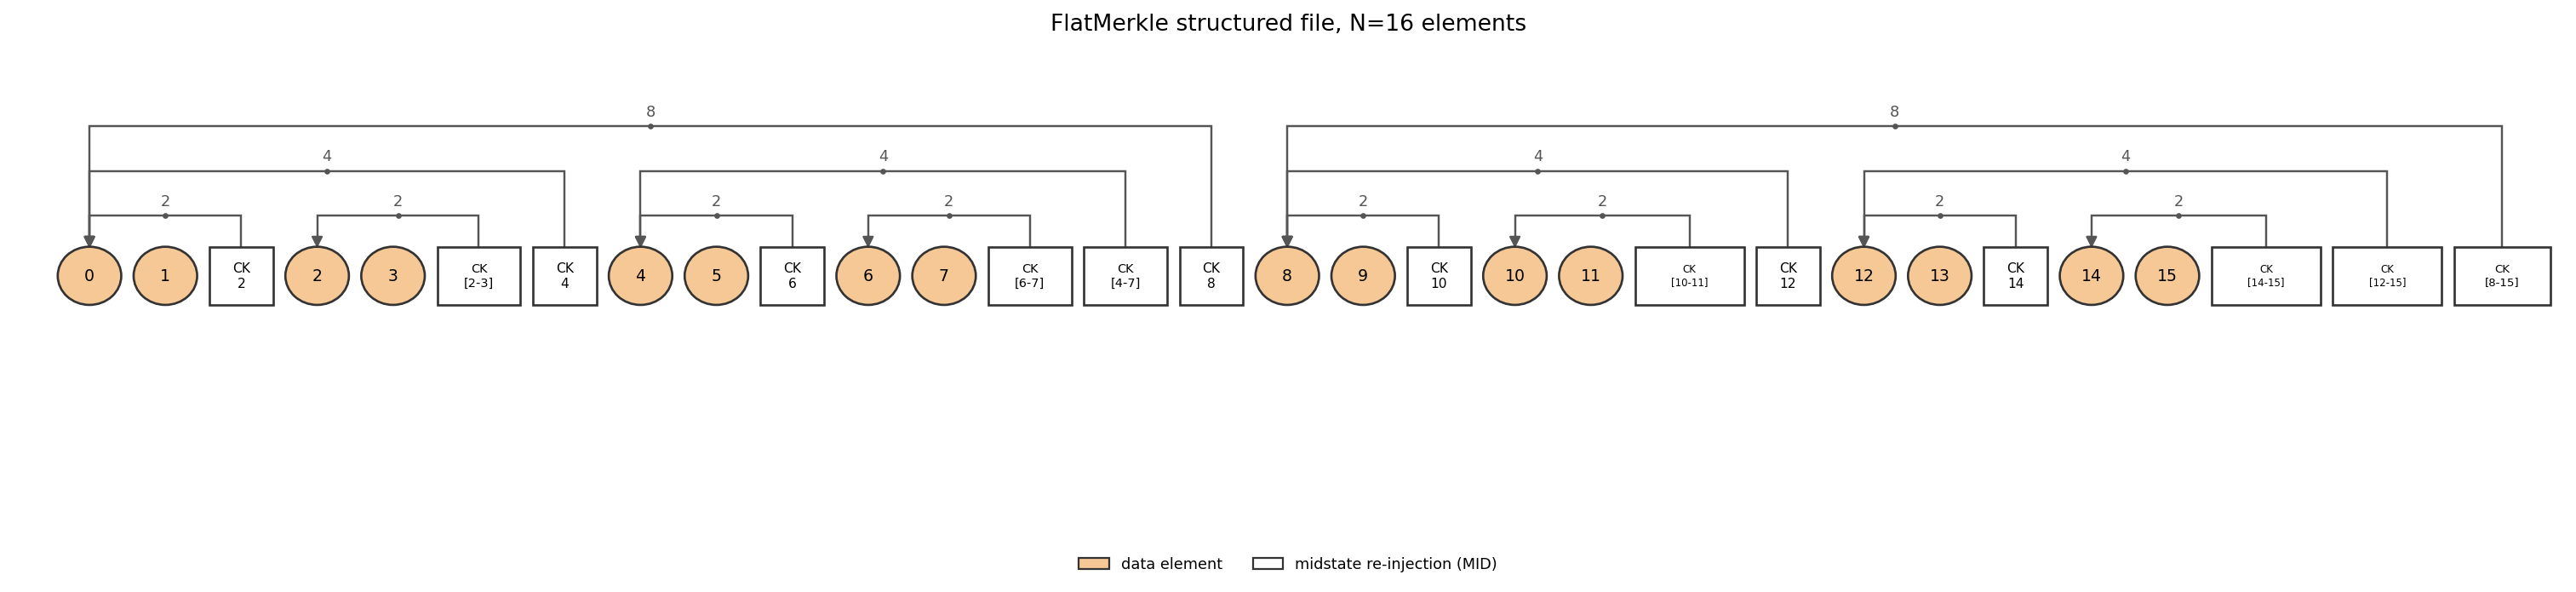
\includegraphics[width=\textwidth]{figures/structure_n16_plain.png}
\caption{The structured file for $N=16$ elements, in full: data elements as
circles, $\mathrm{MID}$ (checkpoint re-injection) blocks as boxes labelled
by the rule above, and the distance-$2^k$ jump arcs implicit in the
recursion, drawn above the row with an arrowhead into the element each arc's
checkpoint traces back to. Read each box's label as naming the state that
box's arc points \emph{at} (the state \emph{entering} the block it opens),
not the block immediately to its left: the box labelled $\CK_4$, for
instance, physically \emph{contains} $\CK[0]=\mathrm{IV}$ and its arc points
back at element 0 -- it is promoting that value forward to be the
checkpoint of the block starting four elements later, not describing
anything about its own immediate neighbors.}
\label{fig:structure-n16}
\end{figure}

\subsection{Position formula}

To build or verify a proof for original index $a$ without materializing the
whole file, we need to know exactly where in the structured file's byte
stream element $a$'s content sits.

\begin{lemma}[Position formula]
\label{lem:position}
For any original index $a \in [0, N)$ -- even or odd, not only positions
that start a block -- the 0-indexed position of $D[a]$ in the structured
file is
\begin{equation}
\mathrm{position}(a) = 2a - \popcount(a),
\end{equation}
where $\popcount(a)$ is the number of 1-bits in the binary representation
of $a$.
\end{lemma}

\begin{proof}[Proof sketch]
By induction on the recursive structure of Section~\ref{sec:recursive-structure}.
Every element contributes exactly one data slot; every completed pair
contributes one additional $\mathrm{MID}$ slot, and more generally every
completed block at level $k \ge 1$ contributes one $\mathrm{MID}$ slot for
each level it closes. The number of $\mathrm{MID}$ slots emitted strictly
before position $a$ is exactly the number of block-closing boundaries
crossed on the way to $a$, which -- by the standard correspondence between
binary counter increments and block closures in a doubling recursive
structure -- equals $a - \popcount(a)$. Adding the $a$ data slots already
emitted gives $\mathrm{position}(a) = a + (a - \popcount(a)) = 2a -
\popcount(a)$.
\end{proof}

The prover and verifier of Section~\ref{sec:algorithm} never call
$\mathrm{position}(\cdot)$: they branch only on whether the target lies
below a block's midpoint. The formula is for a party holding only the raw
byte stream, who needs to locate $D[a]$ directly -- for example, to extract
an element from a downloaded Bitcoin annex (Section~\ref{sec:bitcoin-annex})
before building a proof. It is verified in the accompanying code against
the recursive construction for every index at every
$N \in \{4,8,16,32,64\}$.
